\documentclass[12pt,a4paper]{report}
\usepackage[utf8]{inputenc}
\usepackage[english]{babel}
\usepackage{amsmath}
\usepackage{amsfonts}
\usepackage{amssymb}
\usepackage{graphicx}
\usepackage{lmodern}
\usepackage{tocbibind} % for toc, tof in table of contents
\usepackage{parskip}
\usepackage{url}
\usepackage[labelfont=bf]{caption} % for bold "figure 1.1"

% To have '-' instead of bullets in the itemize environment
\def\labelitemi{--}

% For hyperlinks and meta data
\usepackage{hyperref}
\hypersetup{
    bookmarks=true,         % show bookmarks bar?
    unicode=false,          % non-Latin characters in Acrobat’s bookmarks
    pdftoolbar=true,        % show Acrobat’s toolbar?
    pdfmenubar=true,        % show Acrobat’s menu?
    pdffitwindow=false,     % window fit to page when opened
    pdfstartview={FitH},    % fits the width of the page to the window
    pdftitle={Simulation of complex actuators},    % title
    pdfauthor={Hubert Woszczyk},     % author
    pdfsubject={Master thesis},   % subject of the document
    pdfcreator={TexMaker},   % creator of the document
    pdfproducer={ULg}, % producer of the document
    pdfkeywords={robotics, physics, bullet, blender, vrep, robocup}, % list of keywords
    pdfnewwindow=true,      % links in new PDF window
    colorlinks=true,       % false: boxed links; true: colored links
	linktocpage=true,    
    linkcolor=red,          % color of internal links (change box color with linkbordercolor)
    citecolor=blue,        % color of links to bibliography
    filecolor=magenta,      % color of file links
    urlcolor=cyan           % color of external links
}

% Margins
\usepackage[left=4cm,right=2cm,top=2cm,bottom=2cm]{geometry}

% For nice tables
\usepackage{booktabs,tabularx}
%\usepackage[tableposition=top]{caption}
%\captionsetup[table]{singlelinecheck=off}

\usepackage{cleveref} %should be the last package

\begin{document}

\begin{titlepage}


\begin{center}
\large
University of Liège - Faculty of engineering
\end{center}

\vfill

\begin{minipage}{0.5\textwidth}

\includegraphics[width=0.9\textwidth]{figures/ULg_logo_couleur.pdf}
\end{minipage}
\begin{minipage}{0.5\textwidth}
\huge
\textbf{Master thesis}\\\\
\normalsize
\textbf{Simulation of complex actuators}\\\\
Author : Hubert Woszczyk\\
Promotor : Pr. Bernard Boigelot\\
\end{minipage}

\vfill
\begin{center}
\large
Master thesis conducted for obtaining the\\ Master's degree in Electrical Engineering\\ by Hubert Woszczyk\\
\vspace*{8cm}
\normalsize
Academic year 2015-2016
\end{center}

\end{titlepage}

\newpage\null\thispagestyle{empty}\newpage

\thispagestyle{empty}
\begin{center}
    \Large
    \textbf{Simulation of complex actuators}
    
    \vspace{0.4cm}
    \large
    Hubert Woszczyk, under the supervision of Pr. Bernard Boigelot
    
    \normalsize
    Academic year 2015-2016\\
    Faculty of Applied Sciences\\
    Electrical Engineering
    
    \vspace{0.9cm}
    \textbf{Abstract}
\end{center}
The word \emph{robot} has been crafted by Czech writer Karel Čapek in his play R.U.R. (Rossum's Universal Robots) in the beginning of the XXth century and is derived from the slavic world \emph{robota} which means \emph{labour} or \emph{work}.


\clearpage
\pagenumbering{roman}
\setcounter{page}{1}
\chapter*{Acknowledgements}
My first thanks go to Prof. Bernard Boigelot who made it possible for numerous students, including me, to work in the passionate field of robotics. I also wish to thank him for his guidance, help and accessibility.

I am deeply grateful to my friends Elodie and Laurine for reading and correcting this manuscript. I also want to thank fellow students Grégory Di Carlo and Guillaume Lempereur with whom I had the pleasure of working together one last time.

Finally, I would like to express my sincere thanks to all those who helped me complete this master thesis.

\tableofcontents

\listoffigures

\listoftables

%% Intro
\clearpage
\setcounter{page}{1}
\pagenumbering{arabic}
\chapter{Introduction}
\section{Context}
For the last ten years, students from the Montefiore institute have been participating in a robotic contest named \emph{Eurobot}, a competition in which wheeled robots battle each other for points in various play environments. After some success and following a thirst for new challenges, it was decided to move on to another contest, \emph{RoboCup}.

\begin{figure}[htp]
\center
\begin{subfigure}[b]{0.45\textwidth}
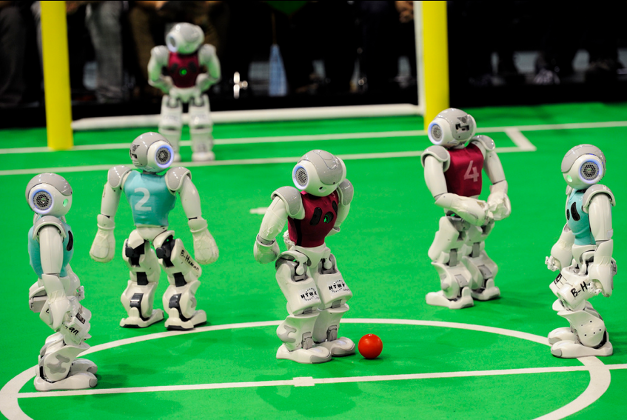
\includegraphics[width=\textwidth]{figures/intro_standard}
\caption[RoboCup Soccer standard platform]{Two teams of Nao robots playing against each other in the 2014 edition of RoboCup Soccer standard platform league. \textit{[Photo courtesy of RoboCup]}}
\label{fig:intro_standard}
\end{subfigure}
\hfill
\begin{subfigure}[b]{0.45\textwidth}
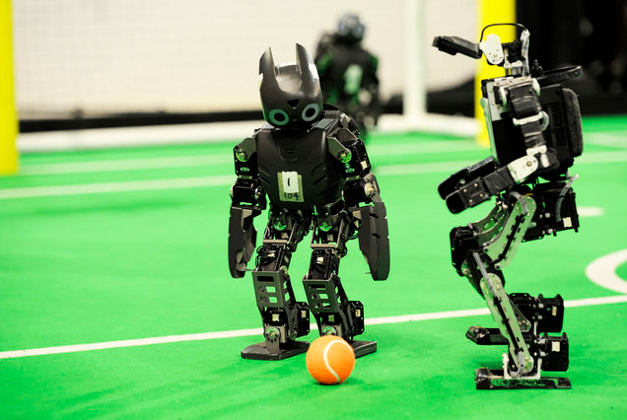
\includegraphics[width=\textwidth]{figures/intro_ks}
\caption[RoboCup Soccer standard platform]{Two robots of opposing teams looking at the ball, in the 2013 edition of RoboCup Soccer kidsize league. \textit{[Photo courtesy of RoboCup]}}
\label{fig:intro_ks}
\end{subfigure}
\caption[RoboCup standard and kidsize leagues]{Robocup standard and kidsize leagues}
\label{fig:intro_robocup}
\end{figure}

This contest is quite vast and, as of 2016, is divided into several categories (called domains in RoboCup jargon):
\begin{itemize}
\item RoboCup Rescue: as the name suggests, a domain where robots must perform various rescue operations in diverse scenarios.
\item RoboCup Industrial: a category with industrially oriented competitions.
\item RoboCup@Home: centred around domestic robots, such as robotics helpers for the elderly or robotic butlers.
\item RoboCupJunior: more of an initiative that aims to foster robotics interest in children rather than a contest, it helps organize various robotics events for younger minds.
\item RoboCup Soccer: historically the first category, centred about humanoid robots playing football. The objective of this category is to have a team of robots beat the world champions by 2050. This is the category we will compete in.
\end{itemize}

RoboCup Soccer is further subdivided into 4 sub-categories called leagues:\begin{itemize}
\item Standard platform, where the teams all use the same robot, \emph{Nao}, as illustrated in \Cref{fig:intro_standard}.
\item Simulation, a league that does not feature physical robots but focuses on team strategies and artificial intelligence. The matches take place in 2D or 3D simulators.
\item Adultsize, for the taller robots.
\item Teensize, for middle sized robots.
\item Kidsize, for the smaller robots. \Cref{fig:intro_ks} shows a match in progress from that league.
\end{itemize}

This year's team is preparing to participate to the Kidsize league and this master's thesis, along with two others, is the by-product of that team's activity. Since this is our first time participating we have no experience regarding humanoids robots. To avoid spending countless hours building and testing different designs we need a tool able of simulating a robot model and its interactions with a physical world.  

\section{Goals of the project}
The goal of this thesis is to provide the team with a physics simulating tool with the following features:
\begin{itemize}
\item realistic simulation of the physics of rigid bodies. This means that the tool should handle inertia, collisions, friction and constraints between objects. Simulation of springs and dampers is an interesting bonus.
\item receive and process orders incoming at a relatively high frequency. The processing need not be in real-time.
\item the model of our robot should receive the same orders as the real robot would. That is, the simulator should provide the same interface to the control code as the real robot would. 
\item 3D visualization of the simulation.
\end{itemize}

That simulator will be used to:
\begin{enumerate}
\item Test different robot designs and choose the best one, in a more efficient way than it could be achieved by physically building the designs.
\item Speed up development and testing of the control code because multiple teams will be able to work in parallel. 
\end{enumerate}

\section{Structure of the report}
This report begins with an overview of the basic concepts behind physics simulation on computers in \cref{chap:principles}. We then move on to \cref{chap:choice} that explains the problem we want to solve and motivates the choice of V-Rep as the main simulation tool for this project.

\Cref{chap:modelling} is about the modelling of our humanoid robot in preparation for \cref{chap:simulation} to go into the core of the subject with some simulations. \Cref{chap:simulation} also explains how our work influenced the design of the robot.

\Cref{chap:conclusion} concludes this work by summing up what is achieved and laying out future prospects.

%% Pre-work
\chapter{Principles of simulation}
In this chapter we discuss the choice of V-rep as the simulation tool for this project. We begin by explaining the basics of rigid body dynamics simulation, take a survey of some of the existing simulators and finally test some of them.

\section{Principles of rigid body dynamics simulation}
The section is heavily inspired by \cite{bender2014interactive}.
The basic idea behind the simulation of physics on a computer is to discretize time and apply the laws of newton to each object in the scene and integrate their acceleration during the timestep. When objects collide, collision.

A rigid body is an idealized solid object which will never change its shape, even under high forces.

The list of physics simulating engines is quite long, but the most popular ones are, in no particular order :
\begin{enumerate}
\item Bullet
\item ODE
\item DART
\item Simbody
\item PhysX
\item Havok
\end{enumerate}

\begin{table}[htp]
\center
\begin{tabularx}{\textwidth}{@{} X X X X X X @{}}
\toprule
\textbf{Engine} & \textbf{License} & \textbf{Coordinates} & \textbf{Origin} & \textbf{Editor} &\textbf{Solver type}\\ 
\midrule
Bullet & Free & Maximal & Games & Blender & Iterative \\ 

ODE & Free & Maximal & Simplified robot dynamics, games & & Iterative\\ 

DART & Free & Generalized & Computer graphics, robot control & &\\

Simbody & Free & Generalized & Biomechamics & \\

PhysX & Proprietary & Maximal & Games & \\

Havok & Proprietary & Maximal & Games & \\
\bottomrule
\end{tabularx}
\caption{Features comparison\cite{engines_comparison}}
\label{table:specs}
\end{table}

\section{Available simulators}
An integrated simulation tool is preferred over a bare-bones physics engine because :
\begin{itemize}
\item time would be lost on creating 3D visualization
\item time would be lost on writing code to import model
\item time would be lost on debugging
\end{itemize}
and all that before the actual work could begin.

\textbf{Blender\cite{Bruyninckx04}
} : \begin{itemize}
\item Uses the Bullet engine
\item Scripting via Python, remote control possible through socket
\item Very complete modelling tool, in a class of its own.
\item Comment : Hard to use because of obscure simulation options and difficulties to correctly set inertias
\end{itemize}

\textbf{Gazebo} : \begin{itemize}
\item Can use Bullet, Simbody, DART or ODE.
\item Scripting via C++
\item Uses SDF format for models.
\item Comment : Hard to use because model must be in SDF format, which no CAD excepted 3dworks exports to. Furthermore, compiled language takes longer to test.
\end{itemize}

\textbf{V-Rep}: \begin{itemize}
\item Can use Bullet, Newton or ODE.
\item Internal scripting in LUA, provides remote API class.
\item Can import 3D collada models.
\item Comment : Best tool so far because model can be imported and the inertias are easy to control, simulation options as well.
\end{itemize}

\textbf{Matlab}: \begin{itemize}
\item Analytical modelling
\item Mathcode
\item No visualization
\item Comment : Not adapted because tedious modelling and no visualization and hard to handle friction and difficult to handle other objects.
\end{itemize}

\begin{table}[htp]
\center
\begin{tabularx}{\textwidth}{@{} l l X X X X @{}}
\toprule
\textbf{Simulator} & \textbf{License} & \textbf{Physics engine(s)} & \textbf{Integrated editor} & \textbf{Modelling}\\ 
\midrule
Blender & Free & Bullet & Fully fledged & Internal\\ 

V-REP & Free (educational license) & Bullet, ODE, Newton, Vortex(10s limit) & Limited & Can import .COLLADA\\

Gazebo & Free & Bullet, ODE, Simbody, DART & Limited & SDF format\\

Webots & Proprietary & ODE & None & SDF format\\

Matlab & Proprietary & None & None & Mathematical\\
\bottomrule
\end{tabularx}
\caption{Comparison of simulators}
\label{table:simulators_comp}
\end{table}

\section{Choice}
Out of Gazebo, V-Rep and Blender, V-Rep is chosen as the best tool because\begin{itemize}
\item Gives the choice between 3 engines, something blender cannot do
\item Makes it easier than Gazebo to create models, because Gazebo uses the URDF format
\item Gives better access than blender to the physical options of the simulation (intertias, timestep of engine)
\item It is multi-platform. 
\end{itemize}

The physics engine used is Newton Dynamics because simple tests showed it to be the most stable with a high number of joints, with the exception of Vortex but it requires a license to run more than $10s$.

While Blender is not used as the primary simulation tool, it is used in the early phases of the modelling because it is what it does best. More on it in the next chapter. 

\chapter{Choosing the tools}
In this chapter we present the problem we want to solve with the simulator and present some of the most popular simulation tools we surveyed. We finally choose one that fits our needs.

\section{Problem statement}
Our robot will consist a number of servos connected together through frames in addition to a central plate that will contain the electronics. We also plan to use spring dampers in the legs to mimic human movement more.

If we want to simulate it we thus need a tool that handles:\begin{itemize}
\item inertia, to have physically accurate dynamics.
\item joints to have constraints between objects.
\item collision and friction, to accurately model the interaction of the feet with the ground.
\item spring dampers.
\end{itemize}

The robot will also have several captors such as accelerometers, rotary position encoders in the servos and we also want to model them in the simulator as they are used by the control algorithms.

We will also have cameras on the robot, therefore if we want to take a holistic approach we should try to model them as well but it is not a priority. 

The final requirement is that we want to be able to control the robot from outside the simulator.

\section{Barebone physics engines}
The physics engine is the cornerstone of a physics simulation tool. There exist a quantity of them, we present here the most popular ones that have the the following features' set :  multi rigid body dynamics, collision detection, joints (hinge, spring-dampers, generic 6DOF\footnote{DOF : degree of freedom}). 

\begin{enumerate}
\item \textbf{Bullet\footnote{\url{http://bulletphysics.org/wordpress/}}:} As of now, the most popular open source physics engine. Although primarily used in video games it is also used in applications such as Blender, V-Rep or NASA's tensegrity robotics toolkit. 

\item \textbf{Newton\footnote{\url{http://newtondynamics.com/forum/newton.php}}:} Another open source engine, not quite as popular as Bullet and ODE but nevertheless used for commercial games and simulation. 

\item \textbf{ODE\footnote{\url{https://bitbucket.org/odedevs/ode/}}:} Open source, a little older that Bullet. As it was already mature when simulators started to be developed, it is present in a lot of robotics simulation tools (V-Rep, Webots, Gazebo...). It was also designed with games in mind but was influenced by its success in more serious applications.

\item \textbf{PhysX \& Havok:} Both are proprietary engines used primarily for games. They won't be further discussed because their focus is on speed rather than accurateness and as such they cannot be used in a simulation that aims to be realistic, as stated by Erez \textit{et al} in \cite{engines_comparison}.
\end{enumerate}

\section{Simulators}
In this section we will discuss software that provides a higher level interface to the physics engines we presented earlier. That interface usually adds a visualization and some other useful features.
\begin{enumerate}

\item \textbf{Blender\footnote{\url{https://www.blender.org/} [Accessed 21/05/2016]}} is 3D modelling software suite and as such has integrated the Bullet engine to help make more realistic animations. It features the ability to make Python scripts that use that engine to make games or physics simulations. 

It is open source and cross platform.

\item \textbf{Gazebo\footnote{\url{http://gazebosim.org/} [Accessed 21/05/2016]}} was the official simulator of DARPA's Robotics challenge. It features multiple physics engines (Bullet ,Simbody, Dart and ODE), allows custom plugins and uses the SDF format for its models. 

It is open source and runs natively on Linux systems but needs to be compiled in order to run on Windows or OSX.

\item \textbf{V-Rep\footnote{\url{http://www.coppeliarobotics.com/} [Accessed 21/05/2016]}} is another simulator that lets you choose the physics engine(Bullet, ODE, Newton, Vortex) and it also allows custom plugins in the form of LUA scripts. It uses its own format for storing models but can import standard formats(COLLADA, 3ds, etc...).

It is cross-platform and free to use for educational purposes.

\item \textbf{Webots\footnote{\url{https://www.cyberbotics.com/} [Accessed 21/05/2016]}} has virtually the same features as V-Rep.

It is cross platform but not free.

\item \textbf{Matlab} is not a dedicated robotics simulator \textit{per se} but can be used to model the robot analytically and to write simulation code for it. 
\end{enumerate}

A summary of the features of each simulator is present on \cref{table:simulators_comp}.

\begin{table}[htp]
\center
\begin{tabularx}{\textwidth}{@{} l l X X X X @{}}
\toprule
\textbf{Simulator} & \textbf{License} & \textbf{Physics engine(s)} & \textbf{Integrated editor} & \textbf{Modelling}\\ 
\midrule
Blender & Free & Bullet & Fully fledged & Internal\\ 

V-REP & Free & Bullet, ODE, Newton, Vortex(10s limit) & Limited & Can import .COLLADA\\

Gazebo & Free & Bullet, ODE, Simbody, DART & Limited & SDF format\\

Webots & Proprietary & ODE & None & SDF format\\

Matlab & Proprietary & None & None & Mathematical\\
\bottomrule
\end{tabularx}
\caption{Comparison of simulators}
\label{table:simulators_comp}
\end{table}

\section{Tested software}
In this section we try some of the proposals presented previously and give our thoughts on them. We will mainly look at the modelling facilities and the access to the underlying simulation options as all the proposed tools possess the required simulation capabilities and are able to deliver similar looking results.

\subsection{Blender}
Blender is convenient to use because the robot's model can be easily changed inside it and the fact that the scripting language is Python make for faster development. Support for a socket allows an external program to control the simulation and the robot inside it. The internals of the physics are obscured and some interesting object properties, such as inertias, are hard to reach. It is also hard to change the simulation parameters making it difficult to obtain stable results when using a higher number of objects and constraints. Furthermore, support for the game engine, the basis of a simulation project, is uncertain, as stated in this development \cite{blender_roadmap}.

\textbf{Pros :}
\begin{itemize}
\item Easy modelling of the elements.
\item The Python API is well documented.
\end{itemize}

\textbf{Cons :}
\begin{itemize}
\item Bullet's simulation parameters are hidden behind an incomplete interface, making it impossible to modify the timestep or the number of iterations for constraint solving.
\item Friction parameter not a physical value but a value between 0 and 1.
\item Inertias are approximated by the principal values Ixx, Iyy and Izz.
\end{itemize}

\subsection{Gazebo}
Gazebo is attractive because it has the support of DARPA and handles multiple physics engines. The main drawback lies in the modelling of the robot to be simulated. It does feature an internal modelling tool but it is too limited to be usable. That would not be a problem if it could import models easily but that is not the case, it uses an xml file to store the parameters of the robot and the only tool that can export models to that format is 3ds max, a commercial product. The team behind Gazebo seems to be well-aware that this is an issue since as of May 2015 it is focusing on developing an internal model editor.

\textbf{Pros :}
\begin{itemize}
\item Gives the choice of the physics engine.
\item Inertias definable as a matrix.
\item Friction represented in physical values.
\end{itemize}

\textbf{Cons :}
\begin{itemize}
\item Internal model editor prohibitively limited, cannot be used to create a complicated model. It cannot import popular CAD formats.
\item Uses the SDF\footnote{A XML file} format to store models, making it hard to iterate over robot designs.
\end{itemize}

\subsection{V-Rep}
V-Rep also has multiple physics engines available and has a user-friendly interface. It also has an internal modelling tool but there is not much use for it since it allows the import of models in the COLLADA format. It also supports socket communication and even provides code for a client thread in the custom application. The options of the physics engines are also pretty accessible and lots of sensor types are natively supported by the simulator.

\textbf{Pros :}
\begin{itemize}
\item Gives the choice of the physics engine.
\item Inertias correctly definable.
\item Friction represented in physical values.
\item Already used at the university.
\end{itemize}

\textbf{Cons :}
\begin{itemize}
\item Limited internal editor, can hardly be used for modelling.
\end{itemize}

\section{Choice}
\subsection{Simulator}
The first choice to be made is whether we go for a barebone physics engines or a simulator: the former has the advantage of being a highly customizable solution but a simulator provides features a physics engines does not :\begin{itemize}
\item 3D visualization
\item code handling the import of models
\item a remote API
\end{itemize}
All these functionalities would eventually be necessary so a simulator is preferred. 

From the available simulators(Blender, Gazebo and V-Rep) the best seems to be V-Rep. This choice is further confirmed by Ivaldi in \cite{ivaldi2014tools} who shows that V-Rep is the highest noted tools amongst roboticists.

Inside V-Rep, we chose Newton Dynamics as the physics engine because simple tests showed it to be the most stable with a high number of joints\footnote{with the exception of Vortex but it requires a license to run more than $10s$}. That choice is further confirmed by Hummel \textit{et al} in \cite{hummel2012evaluation} where Newton Dynamics is stated to be the best engine when it comes to handling a high number of constraints.

\subsection{Modeller}
Although Blender was not chosen as the primary simulation tool for the project, it shall be used as a modelling tool for the robot, as a complement for V-Rep.

\chapter{Modelling tools usage}
This chapter covers the the modelization of the building blocks of the robot.

\section{Problem statement}
Our robot will be mainly made of servos connected together. We thus need to model the behaviour of a servo. Optionally, it could use springs to store energy when walking. 

\section{Basic Modelling}
\subsection{Convex elements}
A convex element is an element which has a convex shape, that is, all its interior angles are less or equal to $180\degree$. Our humanoid robot will have some number of them since a lot of elements can be approximated as cubes, which are convex.

The modelling consists in creating a mesh with the right dimensions, setting the mass and setting the inertia (V-Rep does not feature matrix inertias, only principal axes inertias). Friction of the material can also be set and will influence how much an object will slide.

\subsection{Concave elements}
A shape is concave if it is not convex. It is not recommended to use concave shapes in a simulation as they make collision detection more expensive and the simulation is generally more unstable. 

Therefore, the modelling consists in approximating such a shape by several convex shapes, linked together.

\section{Applied to the building of a humanoid robot}
\subsection{Feet}
The shape of the feet is not fixed yet but it is safe to approximate them by a convex shape with high friction. 

\subsection{Servos}
The robot will mainly be made from MX-28R servos, manufactured by Dynamixel. Their size and power make them an good choice for a humanoid robot. The goal of this section is thus to reproduce as accurately as possible the behaviour of this servo in our simulation.

The MX-28R outer shape is convex so we can create a convex mesh to model its appearance. Its mass and inertias can be set to $77g$ and 
\begin{align*}
Ixx Iyy Izz = (
\end{align*}

\begin{table}[htp]
\center
\begin{tabularx}{\textwidth}{@{} l l l @{}}
\toprule
& \textbf{Data} & \textbf{Unit}\\ 
\midrule
Weight & $77$ & $g$\\
Dimension & $35.6 \times 50.6 \times 35.5$ & $mm^3$\\
Inertia tensor & $\left(\begin{array}{c c c}
2.26e^4 & 3.68e^1 & -2.13e^2\\
3.68e^1 & 1.29ee^4 & -1.15e^3\\
-2.13e^2 & -1.15e^3 & 1.78e^4\\
\end{array}\right)$ & $g \times mm^4$ \\
Stall torque & $2.5$ & $Nm$\\
Nominal torque & $0.7$ & $Nm$\\
\bottomrule
\end{tabularx}
\caption{Characteristics of a MX-28R type servo. Data taken from \cite{mx_28_manual}}
\label{table:specs}
\end{table}

The torque of the servos is computed from the maximal torque of the DC motor and the reduction ratio of the gears. 
\begin{align*}
Torque &= TorqueMotor \times ReductionRatio\\
&= 3.67e^{-3} \times 193\\
&= 0.7083Nm
\end{align*} 

\subsection{Frames}
The frames in use, FR07-H101 are convex and are thus decomposed into into convex shapes that are linked together. 

\subsection{Cameras}
Cameras are modelled as cubes. Their function is performed by vision sensors handled by V-Rep.

\subsection{Springs}



\chapter{Physical validation}
\section{Experimental set-up}
The set-up consists in :
\begin{itemize}
\item A camera that films the movements of a servo configuration.
\item A simulation of that servo configuration in V-Rep.
\end{itemize}

\begin{figure}[htp]
\center
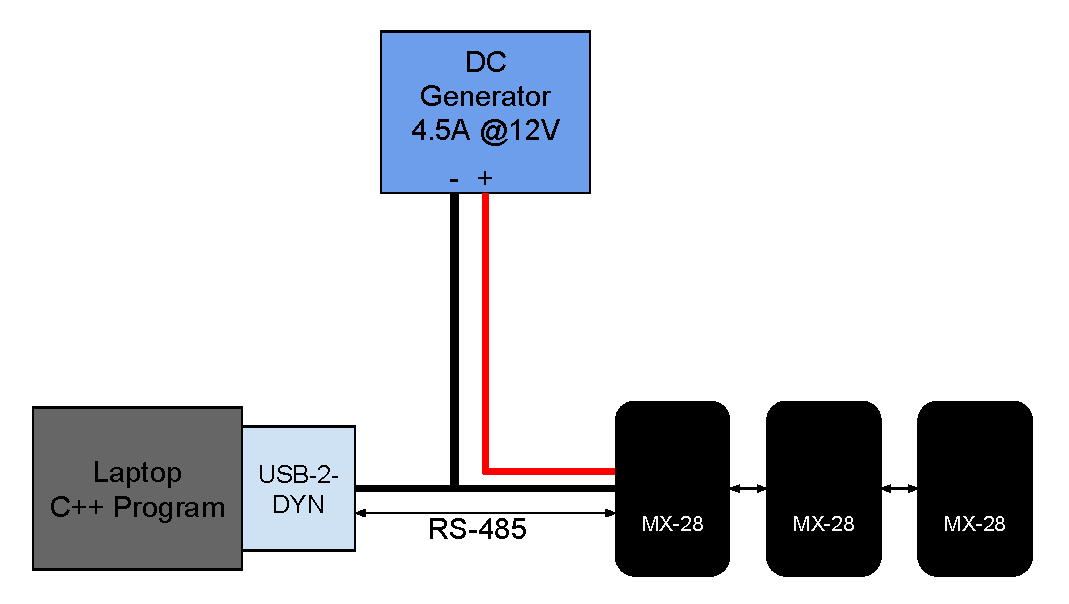
\includegraphics[width=0.6\textwidth]{figures/exp_setup}
\caption{Experimental setup}
\label{fig:exp_setup}
\end{figure}

\section{Experiments}
The first experiment is to test the torque : to that end, a frame is fixed onto a single servo and weighted. The setup is represented on \cref{fig:exp1}.

At $12V$, the maximal torque\cite{mx_28_manual} of the servo is supposedly $2.5N.m$. To test this, a weight of $2kg$ is hanged at $12.5cm$ from the center of the servo, because since 
\begin{align*}
2.5 - 9.81 \cdot (0.007 \cdot 0.01 + 0.016 \cdot 0.0725) &= x \cdot 0.125\\
x &= 20 N\\
&= 2.03 kg
\end{align*}

\begin{figure}[htp]
\center
    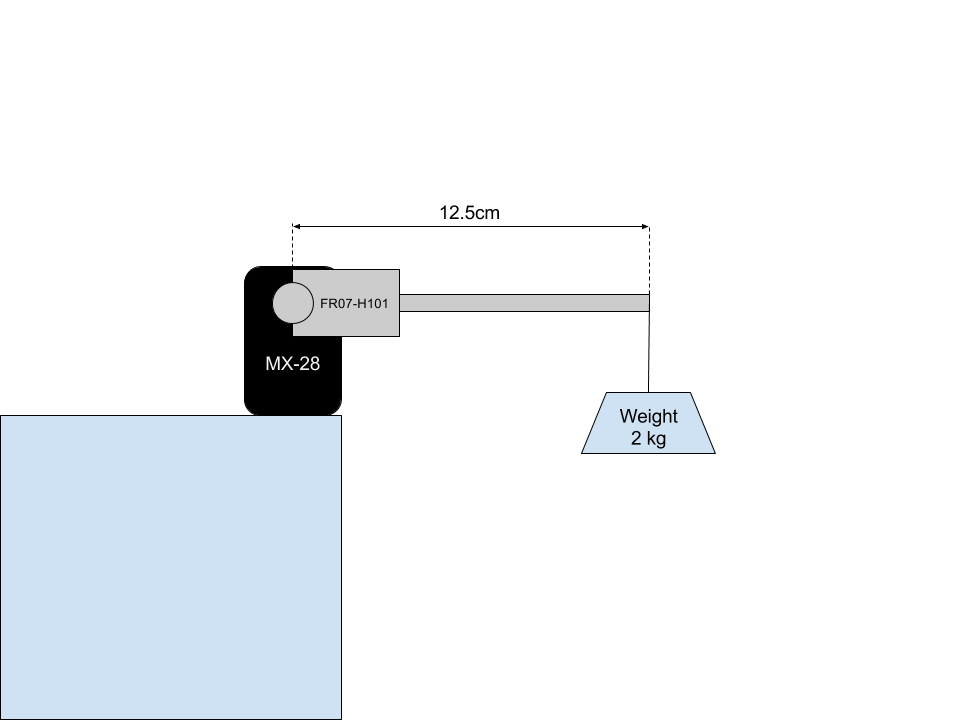
\includegraphics[width = 0.5\textwidth]{figures/exp1}
    \caption[Experimental setup for torque testing]{Experimental setup for torque testing : A weight of $2kg$ is suspended at $12.5cm$ from the servo, resulting in a torque of $2.5Nm$. The goal is to test whether the servo is able to move the weight upwards from the depicted initial situation.}
    \label{fig:exp1}
\end{figure}

Results
\begin{table}[htp]
\center
\begin{tabularx}{\textwidth}{@{}l X X X @{}}
\toprule
& \textbf{Stall torque @11.1V $[N.m]$} & \textbf{Stall torque @12V $[N.m]$} & \textbf{Stall torque @14.8V $[N.m]$}\\ 
\midrule
\textbf{Theoretical} & 2.1 & 2.5 & 3.1\\ 
\textbf{Experimental} &  &  & \\ 
\bottomrule
\end{tabularx}
\caption{Experimental stall torques at different tested voltages}
\label{table:exp1_results}
\end{table}

\section{Servo tuning}

\section{Results}

\chapter{Simulation}
In this section we explain how to use the simulator and how some simulations influenced the design of the robot.

\section{Simulation setup}
The basic idea is to use V-Rep as a simulation platform and use TCP/IP to have another program control the simulation from outside. This gives us great implementation flexibility and we can substitute the real robot by the simulation model easily. This is represented on \cref{fig:simulation_principles}. For this thesis, the control code will be written in MATLAB. 

\begin{figure}[htp]
\center
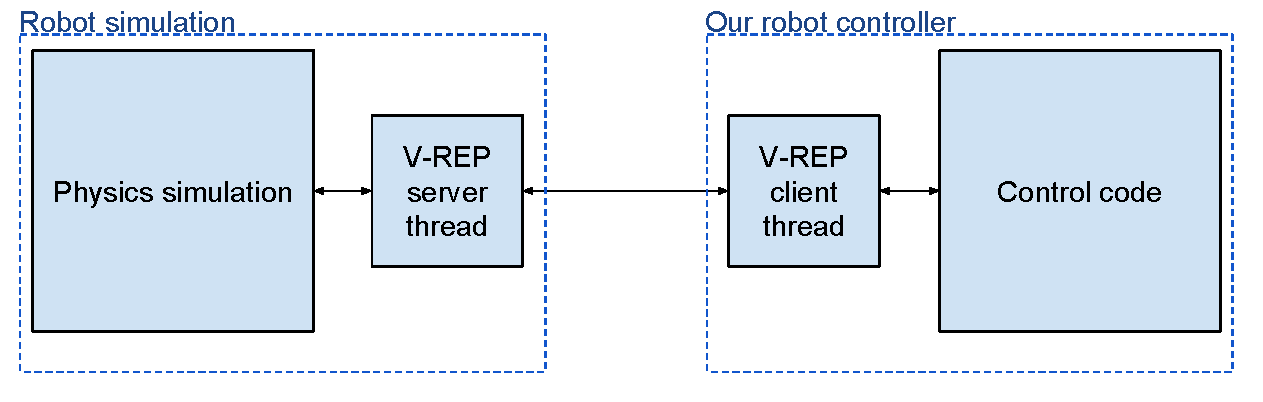
\includegraphics[width=0.6\textwidth]{figures/simulation_principles}
\caption[Simulation principles]{V-Rep simulates the robot while an external program sends order to the robot over TCP/IP thanks to the client/server thread provided by V-Rep.}
\label{fig:simulation_principles}
\end{figure}

Furthermore, the simulation will operate in the synchronous operation mode. That is, each simulation timestep must be triggered by the control code, allowing precise control of the robot. \Cref{fig:remoteApi} presents how V-Rep and the control code interact in synchronous mode.

\begin{figure}[htp]
\center
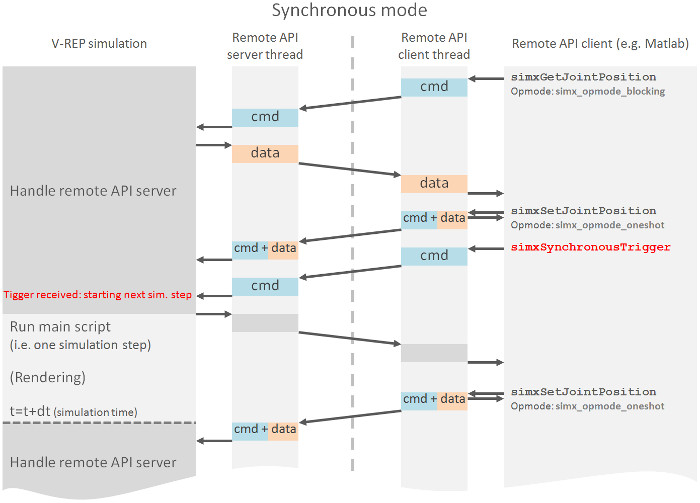
\includegraphics[width=0.6\textwidth]{figures/remoteApiSynchronous}
\caption[Simulation interaction]{Typical interaction between the simulator and the control code. The simulation runs on two threads : the simulation and the server thread. The server threads can receive orders from a client thread which is controlled by a custom application of our own. The simulator waits for a trigger before simulating the next timestep.}
\label{fig:remoteApi}
\end{figure}

\begin{lstlisting}[language=MATLAB, tabsize = 4, float, caption=Basic control program in MATLAB, captionpos = b, frame=leftline, keywordstyle=\color{blue}, numbers = left, commentstyle= \color{mygreen}]
function simulation_client_vrep()
dt = .01;

disp('Program started');
vrep = remApi('remoteApi');
vrep.simxFinish(-1); % close all opened connections
clientID = vrep.simxStart('127.0.0.1', 19997, true, true, 5000, 5);

if clientID < 0
    disp('Failed connecting to remote API server. Exiting.');
    vrep.delete();
    return;
end
disp('Connected to remote API server');

% We close the connexion whenever the script is interrupted.
cleanupObj = onCleanup(@() cleanup_vrep(vrep, clientID));

% This will only work in "continuous remote API server service"
vrep.simxSynchronous(clientID, true);

% retrieve handles to servos, joints
h = robot_init(vrep, clientID);

vrep.simxStartSimulation(clientID, vrep.simx_opmode_oneshot_wait);

i = 1;
while true && t < 3
    instructions = standup_prone(h, t);
    
    i = i + 1;
    send_instructions(vrep, clientID, instructions);
    t = t + dt;
end

% Before closing the connection to V-REP, make sure that the last command sent out had time to arrive.
vrep.simxGetPingTime(clientID);

% Now close the connection to V-REP:
vrep.simxStopSimulation(clientID, vrep.simx_opmode_oneshot_wait);
vrep.simxFinish(clientID);
vrep.delete(); % call the destructor!
disp('Program ended');
end

end
\end{lstlisting}

\section{Applications}
\subsection{Static stability}
The first application is simply to build a model of the robot and test if it is able to stand upright on its own.

The modelling begins in Blender where pieces are simplified/made convex and placed to create the structure of the robot. The model is then exported (in COLLADA) and imported into V-Rep. 

The feet are approximated by a thicker block in order to help with the collision detection. They are also given a high friction.

The torque of the servos is computed from the maximal torque of the DC motor and the reduction ratio of the gears. 
\begin{align*}
Torque &= TorqueMotor \times ReductionRatio\\
&= 3.67e^{-3} \times 193\\
&= 0.7083Nm
\end{align*}
In \cref{sec:exp1} we determined that the maximum torque the servo was actually able to produce was $1.7Nm$ so to represent this we choose to set the maximum torque of the servos to $1Nm$.

In V-Rep the different elements of the robot are dynamically enabled and given mass, accordingly to the values listed in \cref{table:weights}. Then, joints (motor controlled with control loop activated) are added to simulate the behaviour of the servos. Their maximal torque is set to $1.6$, the maximum torque developed my Mx-28 servos as shown by our earlier experiments (\cref{table:exp1_results}). 

\begin{table}[htp]
\center
\begin{tabularx}{\textwidth}{@{} l X X l @{}}
\toprule
\textbf{Module} & \textbf{Weight [$g$]} &  \textbf{Density [$kg/m^3$]}& \textbf{Dimensions [$mm \times mm \times mm$]}\\ 
\midrule
Odroid C-2 & 40 &  & 85.0 x 56.0 x 10.0\\
Li-Po battery & 188 & 2304 & 103.0 x 33.0 x 24.0\\
Mx-28R & 72 & 1150 & 35.6 x 50.6 x 35.5\\
LI-USB30-M021C & 22 & 2200 & 26.0 x 26.0 x 14.7\\
Frame Fr-07 & & 1200 & \\
Frame Fr-101-H3 & 7 & 1200 & \\
\bottomrule
\end{tabularx}
\caption[Weights and dimensions of the pieces of the robot]{Weights and dimensions of the pieces of the robot. The density is useful for the automatic computation of the weight and inertia of the pieces in V-REP.}
\label{table:weights}
\end{table}

The springs on the leg are simulated by two spherical joints and one prismatic joint set to spring-damper mode.

The servos of the robot are simply ordered to hold their initial angle and the simulation determines that the robot can indeed stand upright without any active stabilization.

\subsection{Standing up routines}
This section is heavily inspired by \cite{Stuckler06}

\subsection{Walking}

\section{Influence on robot's design}
The simulator helped shape the robot through simulations that unveiled serious design problems (inability to stand after a fall, inability to walk).

The first design is visible on \cref{fig:first_robot}. It was plagued by stability problems, overcomplicated arms and simulation difficulties. 
\begin{figure}[htp]
\center
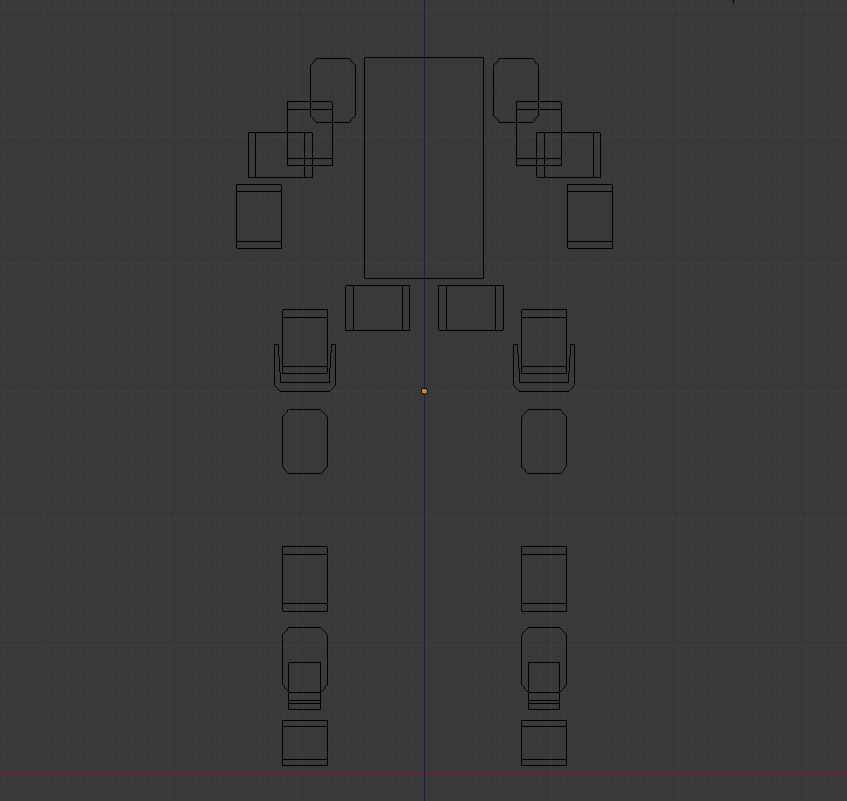
\includegraphics[width=0.6\textwidth]{figures/robot1}
\caption[Initial robot design]{First robot design. Arms use 4 servos each, making it quite heavy.}
\label{fig:first_robot}
\end{figure}

The final design, visible on \cref{fig:final_robot} has better stability, wider movement possibilities and can stand up and walk more easily. 
\begin{figure}[htp]
\center
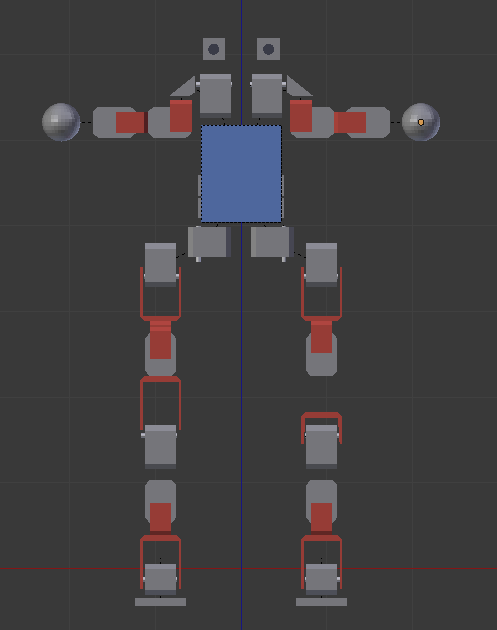
\includegraphics[width=0.6\textwidth]{figures/robot2}
\caption[Final robot design]{Final robot design. Arms now use 3 servos. The feet and the hips use a different configuration to have wider movement possibilities and bring down the center of gravity.}
\label{fig:final_robot}
\end{figure}

The final dimensions of the robot respect the rules of the contest:
\begin{itemize}
\item Height : $61.3cm$
\item Height of COM : $34cm$
\item Height of legs : $cm$
\item Height max is $< 1.5 \times 61.3$.
\item Foot area is $ cm^2$.
\end{itemize}

\chapter{Conclusion}
\section{Problems encountered}
A master thesis is a major endeavour and these are rarely devoid of obstacles. During this year several elements obstructed the completion of this work : \begin{itemize}
\item V-Rep is a fine tool but the lack of a proper internal modelling tool really hindered this work as every major modification meant that the whole model had to be modified in Blender and re-imported into V-Rep. This created a lot of overhead work which contributed nothing of interest to this work. 

This drawback is generalized amongst all the simulators that we surveyed at the beginning of this report and we feel it should be addressed quickly by their creators. Nevertheless, we understand that a modelling tool such as Blender took years to create so we would not expect simulators to catch up any time soon.

\item We also learned of the importance of studying mechanisms carefully before using them. Though things might appear simple at first, subtle implementation details might change everything. A fine example of that is us melting the core of the motor inside a MX-28R servo during our tests because of our trust in the announced safety mechanisms. Needless to say, they proved insufficient and we should have examined the documentation more closely.
\end{itemize}


\section{Future work}
\subsection{Modelling}
As of now it is still uncertain if Blender shall continue to support the COLLADA format (as explained in \cite{blender_roadmap}). In the negative, another tool should be chosen to perform the modelling.

The springs also need some work, as of now they are just there as a proof of concept but their parameters will need to be tuned.

As of now, the model uses simplified inertias, in the belief that a controller should be able to correct minor differences in behaviour between the model and the actual robot. In the case, theses inertias need to be more accurate, we suggest to use Meshlab\footnote{\url{http://meshlab.sourceforge.net/}} to compute the inertias of those objects.

\section{Conclusion}
This is the conclusion to my work.


\bibliographystyle{alpha}
\bibliography{bib}

\appendix
\chapter{Rules}
The robots that participate in the kidsize competition must respect the following characteristics\cite{robocup_rules}:\begin{enumerate}
\item $40cm \leq H_{top} \leq 90cm$.

\item Maximum allowed weight is $20kg$.

\item Each foot must fit into a rectangle of area
$(2.2 \cdot H_{com})^2/32$.

\item Considering the rectangle enclosing the convex hull of the foot, the ratio between the longest side of the rectangle and the shortest one, shall not exceed $2.5$.

\item The robot must fit into a cylinder of diameter $0.55 \cdot H_{top}$.

\item The sum of the lengths of the two arms and the width of the tor
so at the shoulder must be less than $1.2\cdot H_{top}$. The length of an arm is defined as the sum of the maximum length of any link that forms part of the arm. Both arms must be the same length.

\item The robot does not possess a configuration where it is extended longer than $1.5 \cdot H_{top}$.

\item The length of the legs $H_{leg}$, including the feet, satisfies $0.35 \cdot H_{top} \leq H_{leg} \leq 0.7 \cdot H_{top}$.

\item The height of the head $H_{head}$, including the neck, satisfies $0.05 \cdot H_{top} \leq H_{head} \leq 0.25 \cdot H_{top}$. $H_{head}$ is defined as the vertical distance from the axis of the first arm
joint at the shoulder to the top of the head.

\item The leg length is measured while the robot is standing up straight. The length is measured from the first rotating joint where its axis lies in the plane parallel to the standing ground to the tip of the foot.
\end{enumerate}


\end{document}
